\chapter{A Parameter Space Exploration of Dust Formation within WCd Systems Using an Advected Scalar Dust Model}

\begin{abstract}
    
\end{abstract}

\section{Introduction}

% //TODO REWRITE THIS, NOT VERY GOOD!

A Wolf-Rayet star is thought to be a hydrogen depleted OB-type star, as vigorous Triple-$\alpha$ fusion reactions within the core exert massive radiation pressures upon the stars envelope, driving it away in the form of a dense, fast ($\sim 1000 \, \si{km.s^{-1}}$) wind. Through this mechanism, enormous mass-loss rates on the order $10^{-5} \, \si{\solarmass\per\year}$ are produced \cite{crowther_physical_2007}.
Wolf-Rayet stars have multiple subtypes, based on their elemental abundances, WC, which is Carbon abundant, WN, which is Nitrogen abundant, and WO, which is Oxygen abundant. These systems can also be divided into early and late type, depending on the level of Hydrogen depletion.

% Explanation

The WC subtype is of particular importance in this paper, due to its dust producing properties. Despite the extremely high UV flux and wind temperature of these stars ($L_* \gtrsim 10^5 \, \si{\solarluminosity}$, $T_* \gtrsim  40,000 \, \si{\kelvin}$), interstellar dust in significant quantities has been observed in a number of systems. The presence of a binary partner - either OB or WR type - facilitates dust formation through colliding winds, which produce extremely high local densities and a UV-opaque medium conducive to dust formation. % //FIXME use of the phrase UV-opaque isn't particularly good, need a better one.
While a large proportion of WC stars are a part of a binary system \cite{rossloweSpatialDistributionGalactic2015} systems that exhibit colliding wind properties are considerably rarer. % //TODO cite this
Despite this, the massive quantities of dust formed from these systems (between $10^{-10}$ and $10^{-6} \, \si{\solarmass\per\year}$) can substantially affect the local interstellar medium (ISM). 
%//TODO cite this

CWB systems can be described using two important variables, the wind momentum ratio, $\eta$ and the cooling parameter, $\chi$. The wind momentum ratio is fairly self-explanatory, describing how dominant the primary wind is over the secondary. In the case of a WR+OB pair, the WR star is invariably dominant, with the equation taking the form:

\begin{equation}
  \eta = \frac{\dot{\text M}_\text{OB} v^\infty_\text{OB}}{\dot{\text M}_\text{WR}v^\infty_\text{WR}} ,
\end{equation}

where $\dot{\text{M}}$ denotes the mass loss rate of a star, while $v^\infty$ is the terminal velocity of a stars outflow. A low mass loss ratio indicates that the winds are extremely imbalanced, with one star dominating in terms of outflow. As momentum ratio decreases, the apex of wind collision region is pushed towards the secondary star, such that:

\begin{equation}
  r_\text{OB} = \frac{\eta^{1/2}}{1+\eta^{1/2}} d_\text{sep} ,
\end{equation}

where $d_\text{sep}$ is the orbital separation of the binary pair. In the case of a very small wind momentum ratio the primary stars wind completely envelopes the secondary stars forming a strong shock front; the geometry of which can be approximated in the form of a conic surface with an opening angle, $\theta$,

\begin{equation}
  \theta \simeq 2.1 \left( 1 - \frac{\eta^{2/5}}{4}\right) \eta^{-1/3} ~~~ \text{for} ~ 10^{-4} \leq \eta \leq 1 ,
\end{equation}

to a high degree of accuracy \cite{eichler_particle_1993}.

The cooling parameter, $\chi$, compares the cooling time to the escape time from the shock region for a parcel of gas in the immediate post-shock environment. An approximation can be made using the known parameters of a system using the equation:

\begin{equation}
    \chi = \frac{t_\text{cool}}{t_\text{esc}} \approx \frac{v_8^4 d_{12}}{\dot{\text M}_{-7}} , 
\end{equation}

where $v_8$ is the wind terminal velocity in units of $10^8$ \si{cm.s^{-1}}, $d_{12}$ is the distance to the WCR apex in units of $10^{12}$ \si{cm}, and $\dot{\text M}_{-7}$ is the mass loss rate in units of $10^{-7} \si{\solarmass\per\year}$ \cite{stevens_colliding_1992}. Small values of $\chi$ indicate that radiative cooling dominates the dynamics of the system, while larger values indicate an adiabatic system. Strong cooling occurs in comparatively slow, dense winds with a high metallicity, as such it can be predicted that the post-shock WR flow will rapidly cool from the immediate post-shock temperature of $10^8 \, \si{\kelvin}$ to temperatures in the dust formation range, $\lesssim 10^4 \, \si{\kelvin}$.

% Dust formation within CWB systems

Dust producing CWB systems have been observed forming dust either persistently or continuously, further observations have noted that systems with persistent dust formation have more circular orbits, while systems with 

Furthermore, dust producing CWB systems are capable of forming dust both persistently or continuously.
Observations of a variety of systems have determined that the dust formation periodicity appears to be dependent on the orbital properties of the system - dust is formed continuously in systems with more circular orbits while periodic dust formation occurs in highly elliptical systems. This suggests that there is a range of parameters that lead to stars producing the conditions necessary to produce dust, and that at certain separations, dust formation can occur.
% //TODO CITE
%//TODO clean up, refer to dust formation stuff in paper 2



% Brief explanation of why this paper is necessary

This paper examines the changes to the dust formation rates of a system as the parameters of the system change. In particular, the orbital properties of the system, the effect of simulated cooling on the system, and changes in the wind momentum ratio by varying mass loss rate. An ideal continuous dust forming WR+OB system is used as a baseline, periodic dust forming systems are beyond the scope of this paper. 


\section{Simulating CWB Systems}

% //TODO CLEAN  UP BACKGROUND ATHENA

% Background of Athena

Our simulations were generated using the Athena++ hydrodynamical code \cite{stoneAthenaAdaptiveMesh2020}, simulations are generated in 3D and the Euler equations of hydrodynamics are solved in the form:


% //FIXME For now I have included the standard Euler equations, need to discuss with Julian as to whether these are the right terms I should be using, might need some right hand terms for dynamic gas cooling

\begin{subequations}
  \begin{align}
    \frac{\partial\rho}{\partial t}+\nabla \cdot \left(\rho \boldsymbol{u}\right) & = 0 , \\
    \frac{\partial \rho \boldsymbol{u}}{\partial t} + \nabla \cdot \left(\rho \boldsymbol{u} u + P \right) & = 0, \\
    \frac{\partial \rho \varepsilon}{\partial t} + \nabla \cdot \left[ \boldsymbol{u} \left( \rho\varepsilon + P \right) \right] & = \dot E_{cool} , 
  \end{align}
\end{subequations}

where $\varepsilon$ is the total specific energy, $\varepsilon = \boldsymbol{u}^2/2 + e/\rho $, $\rho$ is the mass density, $e$ is the internal energy density, $P$ is the gas pressure and $u$ is the gas velocity. $\dot E_{cool}$ is the energy loss rate from the fluid due to gas and dust cooling, which is elaborated on in section \ref{sec:gas-dust-cooling}.

% Technical details

For these simulations Athena++ has been configured to run using a piecewise linear method with either a 3\ts{rd} order Runge-Kutta or 4\ts{th} order Strong Stability Preserving Runge-Kutta time-integration method \cite{spiteriNewClassOptimal2002}. The 3\ts{rd} order method is significantly faster and more memory efficient than the 4\ts{th} order method, so is used if the simulation permits. Athena++ was forked from the original repository and additional routines were written for a Colliding Wind Binary case. A function to produce a steady outflow from a small spherical region around a set of cartesian co-ordinates was incorporated to simulate the outflow of both stars, while a function to move these co-ordinates with each time-step was included to simulate orbital motion. Additionally, Athena++ was further modified to include an advected scalar dust model for simulating dust growth and destruction as well as a photon emission cooling model to approximate cooling for gas and dust particles within the fluid.

\subsection{Mesh refinement}

%//TODO This section is a little choppy!

Simulating a CWB system is a complicated task due to the extremely large range in length scales required to correctly observe the simulation. The initial wind collision region cannot be abstracted into a generic outflow if orbits are to be considered, as the separation of the stars is extremely important to the evolution of the wind collision region. Furthermore, as grain growth occurs over a long time scale, the maximum length scale must be correspondingly large. 

Static mesh refinement is used to improve the effective resolution of the simulation. The region around the orbits of the stars is refined to the maximum level, with the refinement level decreasing further out from the simulation. Simulation extent is determined by the maximally refined region around the stars, extent is doubled for every level between the coarsest and finest levels.

SMR is used instead of Adaptive Mesh Refinement as it has proven to be more reliable within Athena++, as it mitigates unintentional over-refinement and refinement and de-refinement of the same meshblock every time-step, referred to as ``grid-thrashing''. Overall using SMR the simulations are much more numerically stable. As the bulk of the dynamics governing the long-term evolution of the model occur over a small distance from the apex of the WCR, much of the simulation can be run at a lower resolution without affecting the simulation outcome significantly.

% Wind mapping and orbiting

\subsection{Wind mapping and orbits}

Stars are simulated by replacing the values for density, $\rho_R$, energy $E_R$, and momentum, $p_R$ within a small region, this region is typically on the order of 10 cells in radius. This rewrite corresponds to a change in mass and mechanical energy imparted by an outflowing wind, such that:

\begin{subequations}
  \begin{align}
    \rho_R & = \frac{\dot M}{(4 \pi r^2 v_\infty)} \\
    P_R & = \frac{\rho_R}{\mu m_H} k_B T_w \\
    E_R & = \frac{P_R}{\gamma - 1} + \frac{1}{2} \rho_{R} v_{R}^2 \\
    p_{R} & = \rho_R v_{R}
  \end{align}
\end{subequations}

% This may need more explanation, depending on previous equations

where $v_R$ is the wind velocity as it flows radially from the center of the ``remap zone'' and $r$ is the distance from the current cell to the centre of the remap zone. This method produces radially outflowing winds from the ``star'' with an expected density and velocity, whilst being stable against numerical error. Unrealistic behavior can occur if the WCR impinges on remap zone if the wind is extremely momentum imbalanced, this can be solved by increasing the simulation resolution.

Orbits are calculated by moving the remap zones over time, this is performed by calculating the current position of the zones using Kepler's laws, this is simple, and makes orbits behave extremely consistently. In order to calculate these orbits, the orbital period, eccentricity and stellar masses are required in the input file.

% Plasma and dust cooling

\subsection{Gas and dust cooling} \label{sec:gas-dust-cooling}

Cooling due to photon emission from gas molecules and dust particles s simulated by removing energy from a cell at each timestep. This energy loss is calculated by integrating the energy loss rates using the Euler method; in regions with very rapid cooling sub-stepping is used to ensure that the solution is accurate, the number of sub-steps is determined by comparing the timestep to the cooling time of the region.

Gas cooling is simulated using a lookup table method, the table contains the gas temperature and associated emissivity, $\Lambda(T)$ of the wind at that temperature. In a typically cooling step, the temperature is calculated and a binary search is performed to find the nearest temperature in the lookup table, a linear interpolation step is then performed to find an appropriate value for $\Lambda$. The emissivity is normalised for a $1 \si{cm^{-3}}$ volume with a density of $1 \si{g.cm^{-3}}$, as such, the energy loss can be calculated with the formulae:

\begin{equation}
  \frac{dE}{dt} = \left(\frac{\rho}{m_H}\right)^2 \Lambda_w(T),
\end{equation}

where $\rho$ is the gas density and $m_H$ is the mass of a hydrogen atom. The lookup table was generated by mixing a series of cooling curves generated by MEKAL from the properties of various pure elemental gasses, these are combined based on the elemental abundances of each wind such that:

\begin{equation}
  \Lambda(T) = n_e n_i \sum{X(E) \Lambda_{E}(T)},
\end{equation}

where $n_e$ and $n_i$ are the electron and ion number density of an element, $X(E)$ is the abundance of an element, while $\Lambda_E(T)$ is the cooling parameter of an element. Figure \ref{fig:cooling-curve} details the emissivities of the cooling curves at various temperatures, as well as non-normalised emissivities for each element. Two lookup tables are used in the simulations, based on the elemental abundances of each star. the Wolf-Rayet star uses a WC curve with a high carbon abundance and hydrogen depletion, while the OB star uses solar abundances. The abundances used in this projects simulations are presented in table \ref{tab:abundances}.

\begin{table}[ht]
  \centering
  \begin{tabular}{@{}ccc@{}}
  \toprule
  \multicolumn{1}{l}{} & \multicolumn{2}{c}{X(E)} \\ \cmidrule(l){2-3} 
   & Solar & WC \\ \midrule
  H & $0.705$ & $0.0$ \\
  He & $0.275$ & $0.546$ \\
  C & $3.07 \times 10^{-3}$ & $0.4$ \\
  N & $1.11 \times 10^{-3}$ & $0.0$ \\
  O & $9.60 \times 10^{-3}$ & $0.05$ \\
  Ne & $1.75 \times 10^{-3}$ & $0.0$ \\
  Na & $3.47 \times 10^{-5}$ & $3.47 \times 10^{-5}$ \\
  Mg & $7.10 \times 10^{-4}$ & $7.10 \times 10^{-4}$ \\
  Al & $6.13 \times 10^{-5}$ & $6.13 \times 10^{-5}$ \\
  Si & $8.60 \times 10^{-4}$ & $8.60 \times 10^{-4}$ \\
  S & $3.82 \times 10^{-4}$ & $3.82 \times 10^{-4}$ \\
  Ar & $1.01 \times 10^{-4}$ & $1.01 \times 10^{-4}$ \\
  Ca & $6.15 \times 10^{-5}$ & $6.15 \times 10^{-5}$ \\
  Fe & $1.52 \times 10^{-3}$ & $1.52 \times 10^{-3}$ \\
  Ni & $7.65 \times 10^{-5}$ & $7.65 \times 10^{-5}$ \\ \bottomrule
  \end{tabular}
  \caption{Abundances used for OB and WC stars}
  \label{tab:abundances}
\end{table}

The cooling regime of this code ranges from $10^4$ to $10^9 \si{\kelvin}$, cooling or heating above or below these temperatures are automatically restricted.

\begin{figure}[ht]
  \centering
  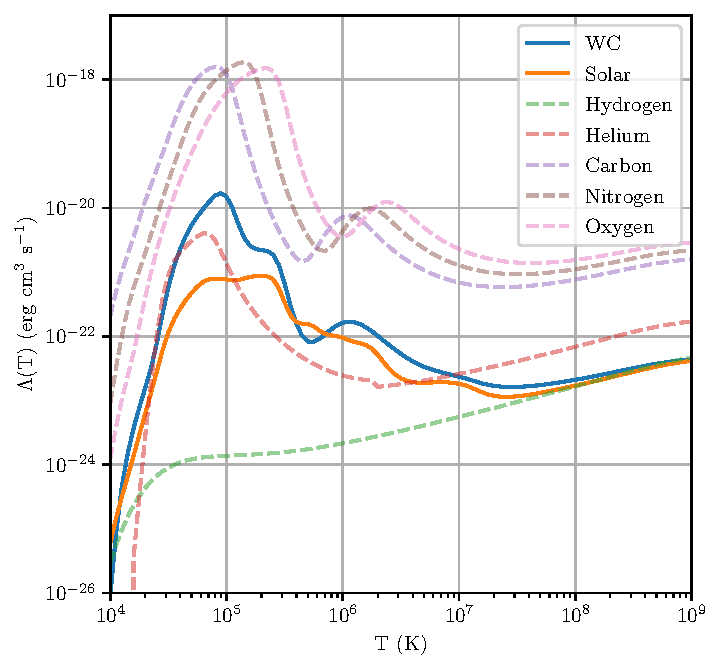
\includegraphics[width=3in]{assets/cooling_curves.pdf}
  \caption[WR and OB $\Lambda(T)$ cooling curves]{Comparison of lookup tables for calculating energy loss due to gas cooling, pure elemental cooling curves from MEKAL have been provided for the more abundant elements.}
  \label{fig:cooling-curve}
\end{figure}

A model for cooling due to emission from dust grains is also included. The rate of cooling is calculated using the uncharged particle case of the Dwek \& Werner prescription \cite{dwek_infrared_1981}. The cooling code simulates grains that are heated due to collisions with ions and electrons, with energy being immediately lost from the simulation as radiation. This assumes that infrared emission due to collisional heating is shorter than the cooling timestep, and the region being simulated is optically thin to far infrared photons. Ions are calculated by element by estimating their number density, and added to the total cooling rate, such that:

\begin{subequations}
  \begin{align}
    H_\text{coll} & = 1.26 \times 10^{-19} \frac{n}{A^{1/2}} a^2(\mu \text m) T^{3/2} h(a,T) , \\
        \Lambda_d & = \frac{H_\text{coll} + H_\text{el}}{n_H} , \\
    \frac{dE}{dt} & = n_T n_d \Lambda_d ,
  \end{align}
\end{subequations}

where $H_\text{coll}$ is the heating rate due to atom and ion collisions, $H_\text{el}$ is the heating rate due to electron collisions, $h(a,T)$ is the particle transparency and $n_T$ is the total number density. $H_\text{coll}$ is summated for Hydrogen, Helium, Carbon, Nitrogen and Oxygen atom collisions. Other elements are not considered as they are present in trivial proportions in both winds.

Electron-grain collisions are modelled similarly to ions, with some differences. In particular, the electron number density needs to be accurately calculated, this is performed with a second series of lookup tables that contain the electron-to-ion ratio of each wind across a temperature range of $10^4$ to $10^9\si{\kelvin}$ (figure \ref{fig:electron-curve}). Additionally, calculating electron transparency is a significantly more complex problem than ion transparency. Electron transparency is calculated via an approximation rather than an integration step, this is used to improve performance, as a time-consuming integration would have to be performed at each cooling substep. The approximation itself is derived from Dwek \& Werner \cite{dwek_infrared_1981}. The approximation for $h(a,T)$ is:

\begin{subequations}
  \begin{align}
    h(a,T) & = 1,              & x* > 4.5 , \\
           & = 0.37x^{*0.62} , & x^* > 1.5 , \\
           & = 0.27x^{*1.50} , & \text{otherwise} ,
  \end{align}
\end{subequations}

where $x^* = 2.71\times 10^8 a^{2/3} (\si{\micro\metre})/T$, this approximation makes the entire dust cooling calculation about 3000\% faster than using a 400 bin integration\footnote{The fastest still reasonably accurate integration.}. Figures \ref{fig:hecomparison} and \ref{fig:lambdacomparison} compare each method, but at high temperatures maximum deviation of the approximation is on the order of $10\%$.

\begin{figure}[t]
  \centering
  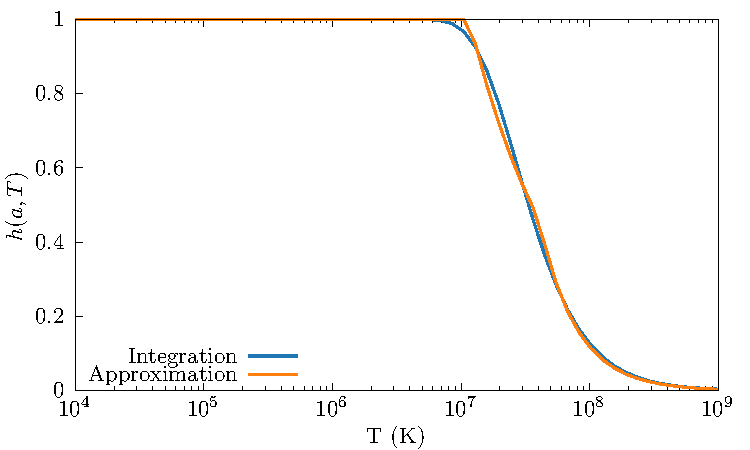
\includegraphics[width=0.8\textwidth]{assets/xe/temp.pdf}
  \caption[Comparison of $h_e$ integration and approximation for increasing gas temperature]{Comparison of $h_e$ integration and approximation for increasing gas temperature, it is clear that the divergence between integration and approximation is at its largest at very high temperatures.}
  \label{fig:hecomparison}
\end{figure}

\begin{figure}[ht]
  \centering
  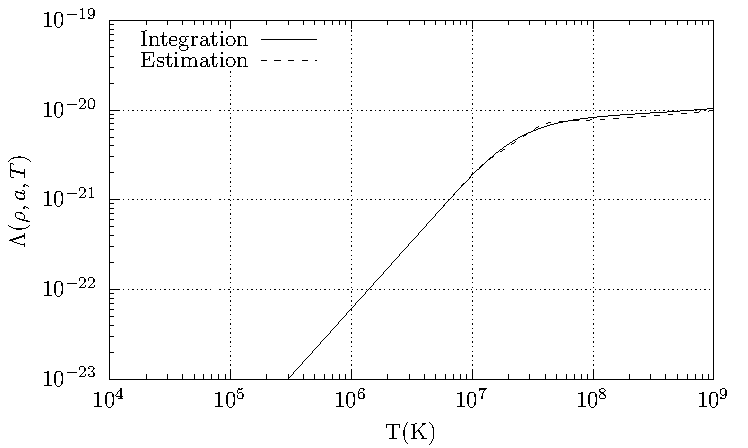
\includegraphics[width=0.8\textwidth]{assets/dustcooling/lambda-comp.pdf}
  \caption[Comparison of dust cooling parameter $\Lambda$(T)]{Comparison of dust cooling parameter $\Lambda(T)$. Error due to approximation does not propagate significantly to the calculation of $\Lambda$ even at high temperatures.}
  \label{fig:lambdacomparison}
\end{figure}


% //TODO Improve caption
\begin{figure}[ht]
  \centering
  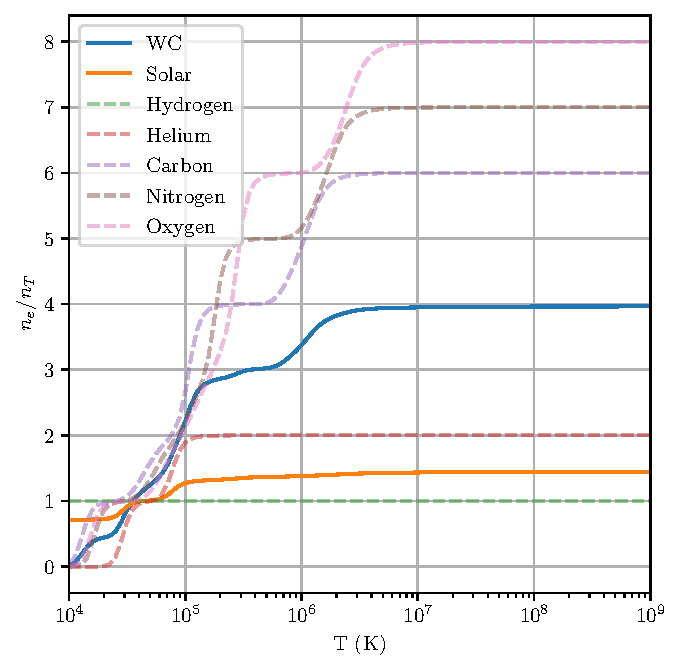
\includegraphics[width=0.8\textwidth]{assets/electron_curves.pdf}
  \caption[OB and WR electron-ion ratios]{A comparison of the electron-ion ratio of both winds as temperature changes, included are the pure wind flows that the lookup tables are built from.}
  \label{fig:electron-curve}
\end{figure}

Grain-grain collision is not modelled, as this would be difficult to calculate due to the single-fluid model in use, further simulations utilising a multi-fluid model could allow for this to be simulated.

% //TODO include a graph of the Wolf-Rayet vs solar abundance ionisation levels.

% Advected scalar modification

\subsection{Numerical modelling of dust through advected scalars}

For this paper a simple dust growth and destruction model was utilised in order to simulate the production of dust within the WCR. Typically a multi-fluid model would be used with a coupling force between the gas fluid and the dust fluid; in this case, however dust is simulated in the form of a set of scalars, which advect according to the fluid dynamics laws governing the simulation. This method emulates the concept of a co-moving fluid, which previous papers have noted is an accurate dynamical model for dust within the WCR \cite{hendrix_pinwheels_2016}. In these simulations, dust is stored in the form of two constants, the average grain radius, $a$, and the dust-to-gas mass ratio, $z$. From these constants the dust production rate, number density, and total dust mass can be derived.

Additionally, a co-moving model allows for a simplified model of dust formation. In such a model, the mean particle velocity between two particles of different size can be given as:

\begin{equation}
  \langle u \rangle = \left[ \frac{8kT}{\pi m_r} \right] ^{1/2} ,
\end{equation}

where $m_r$ is the familiar reduced mass between a test particle of mass $m_t$ and a field particle of mass $m_f$

\begin{equation}
  m_r = \frac{m_f m_t}{m_f + m_t} .
\end{equation}

As the dust grain is significantly more massive, the reduced mass is approximately equal to the grain mass, simplifying the dynamics of the simulation in a co-moving case \cite{spitzer_jr._physical_2008}.

Dust growth is modelled through the method described by \cite{spitzer_jr._physical_2008}, grains co-moving with a gas perform low-velocity\footnote{Relative to the overall wind velocity} collisions with the surrounding gas, accreting this gas onto the surface of the dust grain. Assuming a single average grain size and grains  the change in average grain radius and total dust mass density

\begin{subequations}
  \begin{align}
        \frac{da}{dt} & = \frac{\xi_a \rho_{Gr} w_a}{4 \rho} , \\
    \frac{\rho_D}{dt} & = 4 \pi a^2 \rho n_D \frac{da}{dt}   , 
  \end{align}
\end{subequations}

where $w_a$ is the Maxwell-Boltzmann distribution RMS velocity, $\xi_a$ is the grain sticking efficiency, $\rho_{Gr}$ is the grain bulk density, $\rho$ is the gas density, $a$ is the dust grain radius, and $n_D$ is the grain number density. In this experiment, $\xi_a$ is assumed to be $10\%$, while a bulk density analogous to amorphous carbon grains of $3.0 \, \si{g.cm^{-3}}$ is used.

Dust destruction is calculated via gas-grain sputtering using the Draine \& Salpeter prescription - a dust grain has a lifespan, $\tau$, which is dependent on the grain radius, as the grain loses radius proportional to its loss in mass; assuming a spherical grain, the rate of change in mass and radius can be calculated such that:

\begin{subequations}
  \begin{align}
           \tau_D & = 1 \, \text{Myr} \times \frac{a}{n_g} , \\
    \frac{da}{dt} & = - \frac{a}{\tau_D} , \\
    \frac{dm}{dt} & = -1.33 \times 10^{-13} a^2 n_g n_d \rho_{Gr} ,
  \end{align}
\end{subequations}

where $n_g$ is the gas number density \cite{draine_destruction_1979}. More in-depth derivations for these equations can be found in the appendix, section \ref{app:accretiondestruction}.

% //TODO cleanup sentence structures

In order to propagate dust through each simulation, a small initial value for the advected scalars is propagated from the remap zones, the grain radius was set to a sensible minimum grain size of $50 \, \text{\AA}$ while the minimum dust-to-gas mass ratio was set to $10^{-6}$, changing $z_{min}$ does not significantly impact the average final dust-to-gas mass ratio of the system as $z$ rapidly increases within the WCR, and only impacts the amount of dust formed outside of the WCR.


\section{Model Parameters}

For this project, a series of simulations were run in order to determine how dust formation varies due changes in orbital separation and wind momentum ratio. A baseline simulation with properties similar to WR98a was created, which is then modified to change either the orbital separation or wind momentum. Orbital separation is modified by changing the orbital period of the simulation, while wind momentum ratio is modified by adjusting the mass loss ratio and wind terminal velocity for each star. For all simulations a common wind temperature of \SI{1e4}{\kelvin} is utilised.

\begin{table}[h]
  \centering
  \begin{tabular}{cccc}
  \hline
  Parameter & WR & OB & Unit \\ \hline
  $M$ & 10.0 & 10.0 & \si{\solarmass} \\
  $\dot M$ & \num{5.0e-6} & \num{5.0e-8} & \si{\solarmass\per\year} \\
  $v_\infty$ & \num{1e8} & \num{2e8} & \si{km.s^{-1}} \\
  $T_w$ & \num{1e4} & \num{1e4} & K
  \end{tabular}
  \caption{Wind properties of the baseline system}
  \label{tab:baseline-windproperties}
\end{table}


\begin{table}[h]
  \centering
  \begin{tabular}{ccc}
  \hline
  Parameter & Value & Unit \\ \hline
  $d_{sep}$ & \num{5.984e13} & cm \\
  $P$ & \num{5.64e7} & s \\
  $e$ & 0.0 &  
  \end{tabular}
  \caption{Baseline system orbital properties}
  \label{tab:baseline-orbits}
\end{table}


\subsection{Wind momentum ratio}

Two sets of simulations were run which varied the wind momentum ratio, the first set of simulations varied $\eta$ by modifying the mass loss rate of each star, while the second set of simulations adjusted the wind terminal velocity of each star. Each set of simulations had each parameter adjusted for both the Wolf-Rayet and OB star, this led to a total of 9 simulations, which are described in table \ref{tab:momrat-param}.

%// Two figures 

\begin{table}[h]
  \centering
  \begin{tabular}{cccccc}
  
  $\dot M_{WR}$ & $\dot M_{OB}$ & $v^\infty_{WR}$ & $v^\infty_{OB}$ & $\eta$ & $\chi_{WR}$ \\ 
  \si{\solarmass\per\year} & \si{\solarmass\per\year} & \si{\km\per\second} & \si{\km\per\second} & & \\ \hline \\ 
  \multicolumn{5}{c}{\textit{Baseline}} \\ \hline
  \num{5e-6} & \num{5e-8} & \num{1e8} & \num{2e8} & 0.02 & 1.049 \\ \\
  \multicolumn{5}{c}{\textit{$\dot M$ adjusted}} \\ \hline
  \num{1e-5} & \num{5e-8} & \num{1e8} & \num{2e8} & 0.01 & 0.544 \\
  \num{2.5e-8} & \num{5e-8} & \num{1e8} & \num{2e8} & 0.04 & 1.995 \\
  \num{5e-6} & \num{1e-7} & \num{1e8} & \num{2e8} & 0.04 & 0.997 \\
  \num{5e-6} & \num{2.5e-8} & \num{1e8} & \num{2e8} & 0.01 & 1.088 \\ \\
  \multicolumn{5}{c}{\textit{$v^\infty$ adjusted}} \\ \hline
  \num{5e-6} & \num{5e-8} & \num{2e8} & \num{2e8} & 0.01 & 17.41 \\
  \num{5e-6} & \num{5e-8} & \num{5e7} & \num{2e8} & 0.04 & 0.062 \\
  \num{5e-6} & \num{5e-8} & \num{1e8} & \num{4e8} & 0.04 & 0.997 \\
  \num{5e-6} & \num{5e-8} & \num{1e8} & \num{1e8} & 0.01 & 1.088
  \end{tabular}
  \caption{Momentum ratio modification parameters}
  \label{tab:momrat-param}
\end{table}

Multiple simulations have similar momentum ratios and cooling parameters, but accomplished via different means, such as changing the secondary star wind rather than the primary. This is done in order to determine whether dust production changes are solely due to these two parameters.

\subsection{Separation distance}

Another series of simulations was performed with a binary pair utilising wind parameters described in table \ref{tab:baseline-windproperties} with a differing orbital separation. Separation was modified by changing the orbital period of each star; in this series, orbital separation was varied from \SI{4}{\au} to \SI{64}{\au} (table \ref{tab:dsep-param}). The main effect of adjusting the orbital radius is the subsequent modification of the cooling parameter, $\chi$, which is inversely proportional to the separation distance. As such, the purpose of these simulations is to confirm that dust formation rate relies strongly on $\chi$, or if there are other factors involved in dust formation. %//TODO clean up

Each simulation has a coarse resolution of $320 \times 320 \times 40$ cells, with a varying number of levels, as the separation distance is doubled, the associated static mesh refinement box is halved and the number of levels is decremented. This manipulation of levels ensures that the number of cells between the stars is kept consistent, reduces memory usage and keeps the average timestep approximately the same.

%//TODO calculate the chi in each simulation
\begin{table}[h]
  \centering
  \begin{tabular}{ccccc}
    \hline
    P & $d_{sep}$ & $\chi_{WR}$ & Levels & Effective Resolution \\
    \si{\second} & \si{\au} &  &  & Cells \\ \hline 
    \num{5.647e7} & 4  & 1.049 & 7 & $20480 \times 20480 \times 2560$ \\
    \num{1.597e8} & 8  & 2.097 & 6 & $10240 \times 10240 \times 1280$ \\
    \num{4.518e8} & 16 & 4.194 & 5 & $5120 \times 5120 \times 640$    \\
    \num{1.278e9} & 32 & 8.388 & 4 & $2560 \times 2560 \times 320$    \\
    \num{3.614e9} & 64 & 16.78 & 3 & $1280 \times 1280 \times 160$    \\
  \end{tabular}
  \caption{Parameters of simulations varying separation distance.}
  \label{tab:dsep-param}
\end{table}



\section{Momentum ratio variation}



\section{Separation variation}




\subsection{Adiabatic flow}


\subsection{Dust production yields}

A clear trend with orbital separation is that dust formation increases drastically as the stars are positioned closer together, at high degrees of separation dust formation ceases, and average grain size drops below the initial value of $50 \text \AA$.

The bulk of dust growth occurs in the immediate post shock region, as dust is rapidly cooled and at a high enough density for dust formation to occur.

This matches observations of episodic dust forming systems, where infrared emission due to dust is maximised at or shortly after periastron passage. This also lends further evidence that dust formation rates are not influenced solely by the momentum ratio, as this is kept constant, and instead is strongly influenced by the wind density at collision and post-shock cooling. 

\subsection{Periodicity within a circular orbit}

Closer orbits were also observed to cause subtle periodic changes, whilst this effect is less pronounced than in a highly eccentric 



\subsection{Wind mixing within the WCR}

%This may need additional work

While interaction between Hydrogen and dust grains is not simulated by the dust model, \cite{leteuffModelDustFormation2002} notes that Hydrogen could be a potential catalyst


% \appendix
% \section{Derivation of Dust Accretion and Destruction Rates}\label{app:accretiondestruction}

% \subsection{Dust destruction}\label{app:destruction}
